\documentclass[UTF8]{ctexart}
\ctexset { section = { format={\Large \bfseries } } }
\pagestyle{plain}
\usepackage{float}
\usepackage{amsmath}
\usepackage{amssymb}
\usepackage{listings}
\usepackage{graphicx}
\usepackage{xcolor}
\usepackage{geometry}
\geometry{a4paper,scale=0.8}
\usepackage{caption}
\captionsetup[figure]{name={Figure}}

\lstset{
language=Python, % 设置语言
basicstyle=\ttfamily, % 设置字体族
breaklines=true, % 自动换行
keywordstyle=\bfseries\color{blue}, % 设置关键字为粗体,
morekeywords={}, % 设置更多的关键字,用逗号分隔
emph={self}, % 指定强调词,如果有多个,用逗号隔开
emphstyle=\bfseries\color{Rhodamine}, % 强调词样式设置
commentstyle=\color{black!50!white}, % 设置注释样式,斜体,浅灰色
stringstyle=\bfseries\color{red!90!black}, % 设置字符串样式
columns=flexible,
numbers=left, % 显示行号在左边
numbersep=2em, % 设置行号的具体位置
numberstyle=\footnotesize, % 缩小行号
frame=single, % 边框
framesep=1em % 设置代码与边框的距离
}

\title{\textbf{Data Structure lab4}}
\author{吴嘉骜 21307130203}
\date{\today}

\begin{document}

\maketitle

\noindent
\textbf {Objective}\\  The objective of this lab is to implement d-ary heaps and analyze their features.\\
\noindent
\textbf {Experiment environment} \\
    Windows 11 VsCode Python 3.10.7 64-bit\\

\setlength{\parindent}{0pt}
A d-ary heap is like a binary heap, but (with one possible exception) non-leaf
nodes have d children instead of $2$ children.
Answer the questions related to d-ary headps below.
\section{}
How would you represent a d-ary heap in an array?\\
\textbf{Answer}:\\
If the root of the heap is at index 0, then:
\begin{itemize}
   \item The parent of a node at index $i$ can be found at index $\lfloor(i-1) / d \rfloor$.
   \item The $j\-th$ child of a node at index $i$ will be at index $d \cdot i + j$ for $j = 1, \ldots , d$.
\end{itemize}
So we can represent a d-ary heap in an array as follows. The root is at index $0$, and its $d$ children at index $i$ are at indices $1, \ldots , d$, and then there are $d$ children for each of those children in order, and so on.
Nodes at depth $k$ (the root node lies at the zeroth depth) will start at index $\sum\limits_{i=0}^{k-1} d^i = \frac{d^k - 1}{d - 1}$ and end at index $\sum\limits _{i=0}^{k} d^i - 1 = \frac{d^{k+1} - 1}{d - 1} - 1$.
To locate the parent or children of a node, we can use the above formulas.
\section{}
What is the height of a d-ary heap of n elements in terms of $n$ and $d$?\\
\textbf{Answer}:\\
For a complete d-ary tree with height $h$, the total number of its nodes is: $1 + d + d^2 + ... + d^h =    
\frac{d^{h+1} - 1}{d - 1}$.\\
So a d-ary heap of n elements with height $h$ satisfies: $\frac{d^{h} - 1}{d - 1} < n \leq \frac{d^{h+1} - 1}{d - 1}$. This leads to
$d^h-1<n(d-1)\leq d^{h+1}-1$  $ \Rightarrow d^h \leq n(d-1) < d^{h+1}$, and that results in $h \leq log_d(n(d-1)) < h+1$\\
$ \Rightarrow h = \lfloor log_d(n(d-1)) \rfloor = \Theta(lg n/lg d)$.

\section{}
Give an efficient implementation of EXTRACT-MAX in a d-ary max-heap. Analyze its running time in terms of $d$ and $n$.\\
\textbf{Solution}: See d\_Extractheapmax.py
\begin{lstlisting}
def extract_max(A,d):
   if len(A) < 1:
      raise ValueError("heap underflow")
   max = A[0]
   A[0] = A[len(A)-1]
   A.pop()
   max_heapify(A,0,d)
   return max

# A: Array
# i: index
# d: d-ary tree
def max_heapify(A,i,d):
   n = len(A)
   child_1 = d*i+1
   child_rightmost = min(d*i+d, n-1) 
   if child_1 <= len(A)-1 and A[child_1] > A[i]:
      largest = child_1
   else:
      largest = i
   for j in range(child_1,child_rightmost+1):
      if j <= len(A)-1 and A[j] > A[largest]:
         largest = j
   if largest != i:
      A[i],A[largest] = A[largest],A[i]
      max_heapify(A,largest,d)
   return A
\end{lstlisting}
\textbf{Analyze}:\\
The EXTRACT-MAX operation involves removing the root, replace it with the last element and then reorganizing the heap. 
The time complexity is dominated by the time to sift down the replacement element to its proper place, which is the running time of MAX-HEAPIFY for d-ary trees.\\
The main change from binary heaps to d-ary heaps is that we need to compare with all $d$ children at each level rather than just two children.
For the worst case, the replacement element will need to be sifted down to the bottom of the heap, which is the height of the heap $\Theta(log_d(n))$, and at every level we need to compare with all $d$ children.
So the worst-case time complexity is: $\Theta(d \cdot log_d(n)) = \Theta(d \ lgn/lgd)$.

\section{}
Give an efficient implementation of INSERT in a d-ary max-heap. Analyze its running time in terms of $d$ and $n$.\\
\textbf{Solution}: See d\_Insertmaxheap.py
\begin{lstlisting}
def max_heap_insert(A,key,d):
   k = float("-inf")
   A.append(k)
   increase_key(A,len(A)-1,d,key)

def increase_key(A, i, d, k):
   if k < A[i]:
      raise ValueError("New key is smaller than the current key!")
   A[i] = k
   while i > 0 and A[parent(i, d)] < A[i]:
      A[i], A[parent(i, d)] = A[parent(i, d)], A[i]
      i = parent(i, d)
   return A
   
def parent(i, d):
   return (i-1) // d
\end{lstlisting}
\textbf{Analyze}:\\
For INSERT operation, the new element is placed at the end of the array with a key of $-\infty$
and then sifted up to its proper position by increasing the key to the desired value.
The running time of INSERT is the same as that of INCREASE-KEY, whose worst case is the element being sifted up to the root, which is the height of the heap $\Theta(log_d(n))$.
Thus, the running time is $\Theta(log_d(n)) = \Theta(lgn/lgd)$.

\section{}
Give an efficient implementation of INCREASE-KEY(A, i, k), which flags
an error if $k < A[i]$, but otherwise sets$ A[i]=k$ then updates the d-ary max-heap
structure appropriately. Analyze its running time in terms of $d$ and $n$.\\
\textbf{Solution}: See d\_Increasekey\_heap.py
\begin{lstlisting}
def increase_key(A, i, d, k):
   if k < A[i]:
      raise ValueError("New key is smaller than the current key!")
   A[i] = k
   while i > 0 and A[parent(i, d)] < A[i]:
      A[i], A[parent(i, d)] = A[parent(i, d)], A[i]
      i = parent(i, d)
   return A
   
def parent(i, d):
   return (i-1) // d
\end{lstlisting}
\textbf{Analyze}:\\
The INCREASE-KEY operation is used to update the value of a key in the heap. The worst-case running time is the height of the heap $\Theta(log_d(n)) = \Theta(lgn/lgd)$.

\section{}
Constructing a 3-ary heap with an insertion sequence ranging from $1$ to $30$,
we shall perform consecutive operations of EXTRACT-MAX and INCREASE-KEY $(A, 10, 28)$, subsequently reporting the results on three occasions.\\
\textbf{Solution}: See 3-ary\_heap\_con.py
\begin{lstlisting}
from d_Buildmaxheap import build_max_heap
from d_Extractheapmax import extract_max
from d_Increasekey_heap import increase_key

# construct a 3-ary heap
A = range(1,31)
A = list(A)
build_max_heap(A,3)
print('The initial 3-ary heap is: ', A)
# extract the maximum element
extract_max(A,3)
print('After one extraction, the 3-ary heap is: ', A)
# increase the key of A[9] to 28
increase_key(A,9,3,28)  # increase the 10-th element
print('After increasing the key of A[9] to 28, the 3-ary heap is: ', A)   
\end{lstlisting}
\textbf{Result}:
\begin{figure}[H]
   \centering
   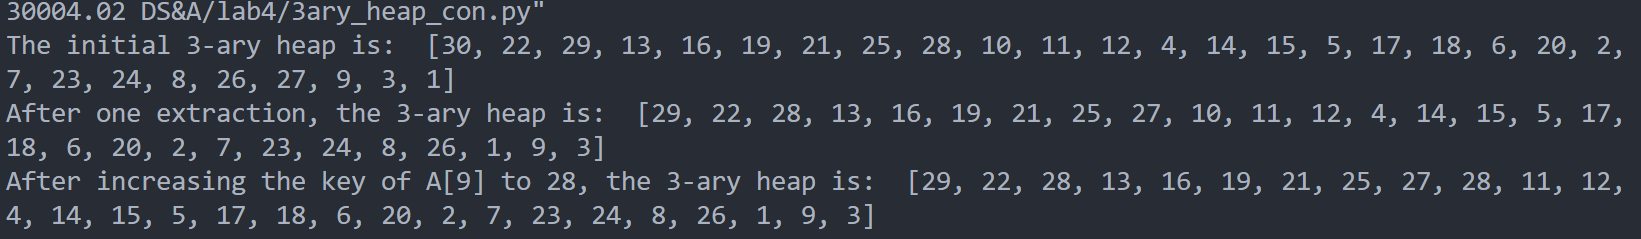
\includegraphics[scale=0.8]{3-ary_heap_con.png}
   \caption{3-ary heap construction and operations}
\end{figure}

\end{document}